\documentclass[11pt]{wbzine}
%packages
\usepackage{lipsum}
\usepackage[utf8]{inputenc}
\usepackage[T1]{fontenc}
\usepackage[ngerman]{babel}
\usepackage{coelacanth}
%\usepackage{imfellEnglish}
%\renewcommand*\sfdefault{ugq}


\begin{document}

\begin{titlepage}
\centering
{\bfseries\fontsize{70}{55}\selectfont Grenzland}

\hrulefill Nummer 1, September 2022
    \vspace{1cm}

	  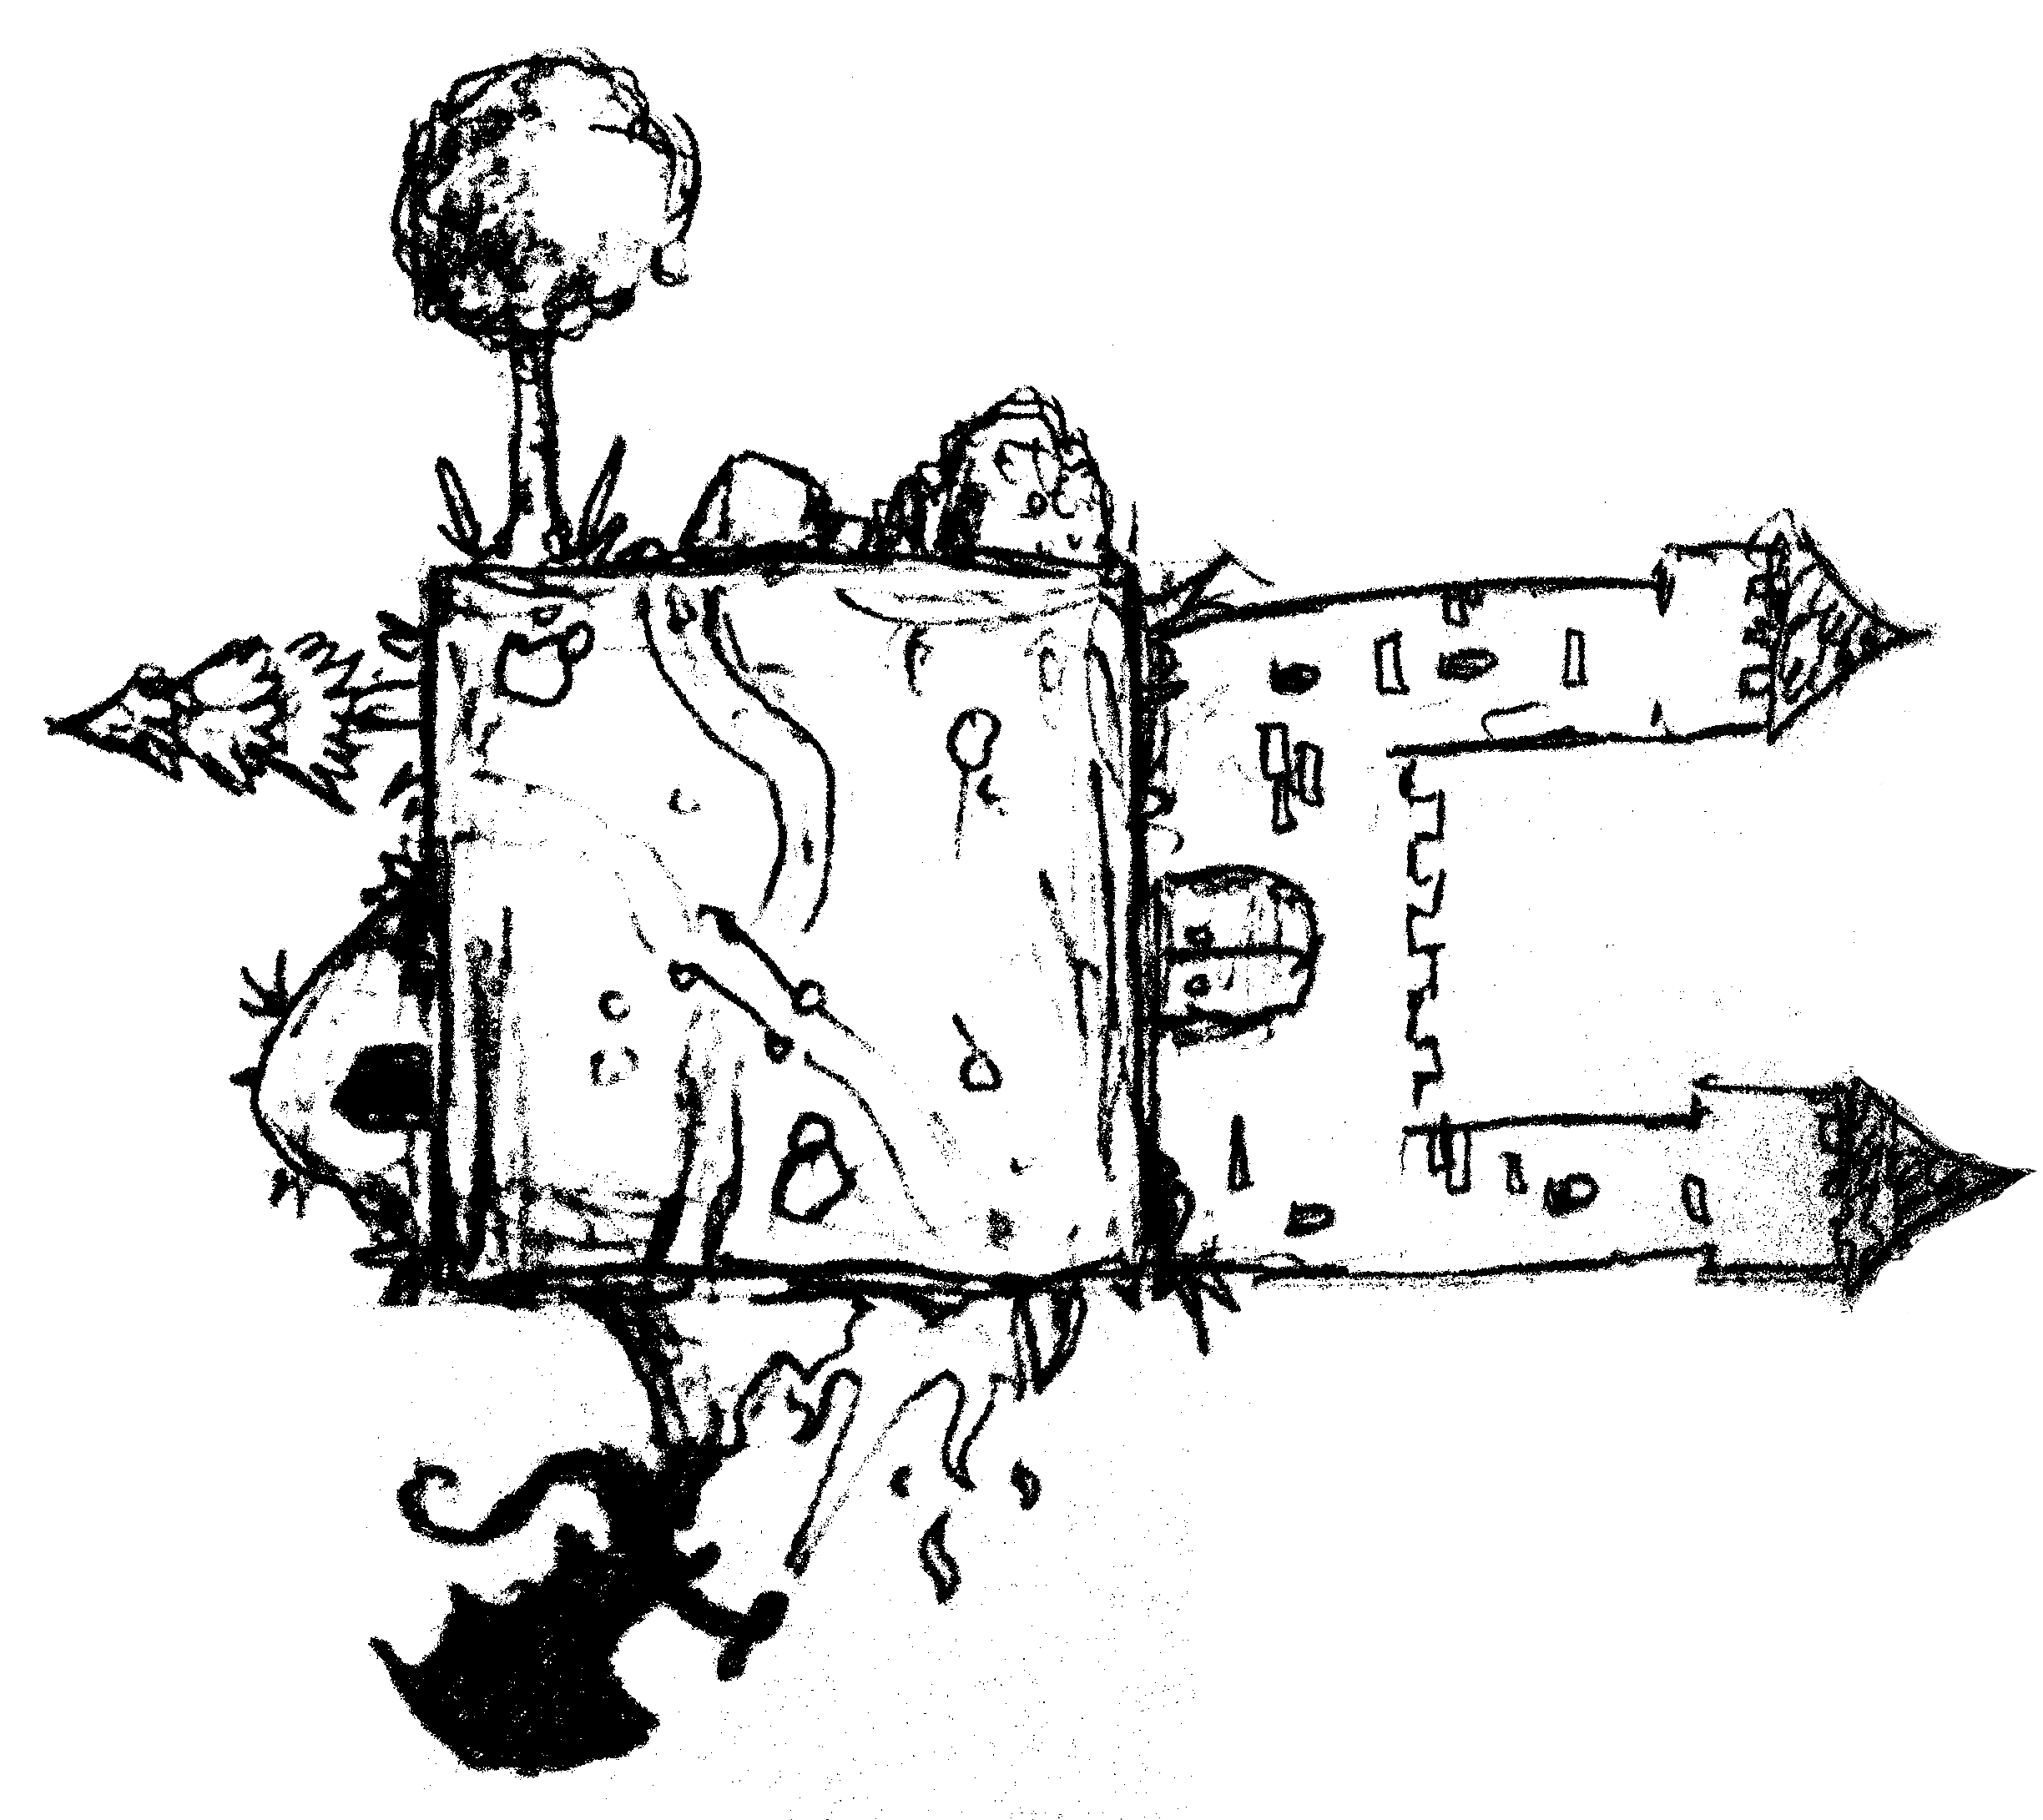
\includegraphics[width=\textwidth]{Coverimage.png}

    \vspace{1cm}
{\Huge Nach dem Kataklysmus\par}%

\end{titlepage}

\tableofcontents

\begin{multicols}{2}

\section{Vorwärts!}
\by{DM Laurens}

Die erste Session der Grenzland-Kampagne wurde am 08.04.2016
    gespielt, die letzte am 23.04.2021. Über diese 5 Jahre spielten
    wir rund 50 Sessions. Zu Beginn in monatlichen Abständen, später
    alle 2 Wochen, und seit Anfang 2021 wöchentlich – immer mit
    einer Sommerpause von Ende April bis Ende September. Rund 20
    Spieler:innen beteiligten sich in wechselnder Konstellation an
    der Kampagne. Rund 30 Charaktere starben im Verlauf der Kampagne
    … oh boy … Die alten D\&D Varianten sind berühmt und berüchtigt
    für ihre ``Tödlichkeit''.

Nun soll es also wieder los gehen. Die Katastrophe, mit der das alte
    Grenzland endete, bietet jetzt, fast zwei Jahre später ein paar
    großartige Anknüpfungspunkte, und löst gleichzeitig ein paar
    Probleme, die ich mit der Kampagnenwelt hatte. Während das alte
    Grenzland auf der veröffentlichten Welt \textit{Mystara}
    beruhte, die viele Ungereimtheiten und einen quasi fest
    geschriebenen Kanon hat, ist das postapokalymptische Grenzland
    neu, anders, und plötzlich etwas eigenes. Und das
    postapokalyptische Grenzland ist nun auch eindeutig unsere Erde
    vor langer langer Zeit. 


Dann also: auf die nächsten 5 Jahre Grenzland!

\section{Was bisher geschah}

Zu Beginn spielten sich die Ereignisse der Kampagne zwischen der
    Festung im Grenzland und den Chaoshöhlen ab. Die Charaktere
    waren ins Grenzland gekommen, um auf Abenteuer auszuziehen, und
    so Ruhm und Gold zu gewinnen. Nicht wenige Charaktere bezahlten
    das mit ihrem Leben, und noch mehr Monster in den Wäldern und
    Höhlen mussten dran glauben. Schließlich überfiel der mächtige
    Drache Darpantor die Festung und die Charaktere waren gezwungen
    die Festung zu verlassen. Sie fanden Zuflucht im zwei
    Tagesreisen westlich gelegenen Hommlet und zogen fortan von dort
    auf Abenteuer aus. Zu Beginn auch noch gelegentlich in die
    Ruinen der Festung, die nun von Dämonen heimgesucht wurde.

Später – in der 4. Spielzeit – begab man sich auf eine Reise in das
    Reich der Zwerge im nördlichen Gebirge. Das Ziel war,
    Handelsbeziehungen mit den Zwergen aufzubauen, und andererseits
    einem der Spielercharaktere bei der Erfüllung ihrer Queste zu
    helfen. Am Ende wurde so ein von dunklen Mächten gefangener
    Golddrache – der ``irdische'' Avatar einer rechtschaffenen
    Gottheit – von den Spielercharakteren befreit, und das Land der
    Zwerge vor dem Verderben bewahrt. 


    Schließlich trat mit der 5. Spielzeit ein seltsamer Kult auf den
    Plan. Die ``Einmonder'' – fanatisch rechtschaffene Kleriker und
    Zauberkundige aus der königlichen Hauptstadt – hatten sich in den
    Kopf gesetzt, einen der beiden Monde, den roten Mond
    Daro aus dem Himmel zu heben, um dadurch dem Chaos ein für alle
    mal Einhalt zu gebieten. Am Ende stellte sich heraus, dass alles
    eine Verschwörung des Drachen Darpantor war. Er hatte 50 Jahre
    zuvor mit einem anderen Drachen gewettet, dass es ihm gelingen
    würde Daro aus dem Himmel zu heben.

\bigmap{Grenzland-praeapo.gen.png}

\bigmap{Grenzland-postapo.gen.png}

    Allein, Darpantor verlor am Ende seine Wette. Den
    Spielercharakteren gelang es zwar nicht, die Einmonder an der
    Durchführung ihres wahnsinnigen Rituals zu hindern, doch sie
    konnten so viel Verwirrung stiften, dass es am Ende Maro, den
    anderen, helleren der beiden Monde traf. Selbst Darpantor, der
    die Wut über sein Scheitern an den Helden auslassen wollte,
    konnte in die Flucht geschlagen werden. Schließlich, durch das
    Zerreißen des Mondes, erschütterten heftige Erdbeben das
    Grenzland, tiefe Erdspalten rissen auf, und verschluckten so
    manchen Abenteurer für immer. Andere wurden auf fremde Ebenen
    gerissen, und nur wenige konnten später von den letzten Tagen
    des alten Grenzlandes berichten.

\subsection{Nach dem Kataklysmus}

Über viele Monate erschütterten immer neue Erdbeben das Grenzland,
und herabstürzende Fragmente des zerstörten Mondes liessen das Land
nicht zur Ruhe kommen. Dicke Staubwolken verdunkelten den Himmel,
und führten zu einer monatelang anhaltenden, eiskalten Nacht. Bis
heute sind große Teile des ehemaligen Grenzlandes unter einer viele
Meter dicken Schicht aus Schutt und grauem Schnee begraben.

Weite Teile des Landes sind durch das Aufbersten gewaltiger Gräben
nicht wieder zu erkennan, und große Teile der Küstenregionen sind für
immer im Meer versunken. Das alte Königreich, das Imperium im Osten,
und die große Wüste sind für immer verschwunden. Dort wo über
Jahrtausende der alte Elfenwald war, erstreckt sich ein riesiger Fjord weit
ins Landesinnere.

Versprengte Gruppen überlebender Völker des alten Grenzlandes ziehen
durch die unwegsamen eiskalten Einöden, auf der Suche nach Nahrung,
Überresten der alten Zivilisation und grüneren Weiden hinter dem
Horizont. Das Leben ist rauh und gefährlich. Gelegentlich können
wertvolle Überreste der alten Zeit gefunden werden, doch die
zahlreichen tiefen Risse in der Erde bergen auch unergründete
Geheimnisse, und Dinge, die seit Äonen unter dem Sediment
der Zeit verborgen waren.

Auch die Inseln des Südens wurden während der letzten Monate immer
wieder von Erdbeeben und Tsunamis heimgesucht, doch die meisten
Menschen haben hier, weit weg vom Epizentrum der Katastrophe,
überlebt. Man sagt die Reiche des alten Festlandes, seien unter den
Trümmern der eigenen Hybris begraben, und junge Menschen machen sich
nun auf, die veränderte Welt neu zu entdecken. Irgendwo weit im
östlichen Ozean, so heißt es, soll gar eine neue Insel geboren
worden sein.
    
\section{Ein harter Marsch}
\by{Oliver}

\textit{Ich mache mir Sorgen wegen des wohl bald kommenden Winters
...}

Die Welt ist nun schon lange nicht mehr so wie sie einmal war. Der
vorletzte Winter fiel komplett aus, wir hatten Temperaturen wie in
einem Hochsommer und ständig konnte man irgendwo Rauch am Horizont
entdecken. Dafür traf es uns im anschließenden Sommer um so härter. 
Dieser war dunkler und kälter als die strengsten Winter, die ich bisher 
erlebt hatte. Nahrung war seitdem knapp. Wir müssen uns vorbereiten,
wenn wir es in den vermeintlich sichereren Süden schaffen wollen.


\textit{Wenn wir damals doch nur Tiberius in der Spalte gefunden
hätten}, schelte ich mich wieder einmal in meinen Gedanken. Mit ihm
wäre uns so einiges leichter gefallen. Ich hatte mich vor zwei
Jahren, nach den schrecklichen Ereignissen mit diesen Spinnern,
natürlich mit Samo umgehend daran gemacht unsere Gefährten
aus den gespenstischen Erdspalten zu befreien. Ich bin mir sicher
das hätte auch geklappt, wenn wir mehr Zeit gehabt hätten. Man hörte
ja noch einige Zeit Geräusche in den Spalten, die man für Hilferufe
in verschiedenen Sprachen halten konnte. Zu Tiberius vermochten wir 
mit unserer Ausrüstung allerdings nicht vorzudringen und 
nach wenigen Stunden rächte sich der weiße Mond und schoss die
Feuerbälle wieder zurück. Das war ein Spektakel und es zeigte sich
das Glück von dem wir Überlebenden profitierten. Keiner der
Feuerbälle traf auch nur bei uns in die Nähe. Aber wir Menschen
hatten scheinbar eine Gottheit erbost. Oder noch so ein dämlicher
Drache trieb sein Spiel mit uns. Jedenfalls riet der weise Samo
dazu, vom Berg abzusteigen und uns in Sicherheit zu bringen. 
Tot würden wir auch niemandem mehr helfen können.


Aber ich schweife ab. \textit{So langsam ist Zeit, dass wir uns einen
Platz für den Winter suchen}, sage ich zu meinen Begleitern die mit
mir bei unserem kargen Abendessen um das Feuer harren. Ich weiß
nicht wie viel weiter südlich wir noch kommen, bis es für unsere
Tagesmärsche zu kalt wird. Es ist aber scheinbar zu spät für das
Gespräch und statt einer Antwort starre ich nur in wortlose,
abgekämpfte Gesichter. \textit{Ich nehme die erste Wache.} 

Vielleicht können wir heute einmal zur Ruhe kommen ...

\section{Ein neues Ziel vor Augen}
\by{Moritz}

Es wurde wirklich Zeit, unser Schicksal wieder in die eigene Hand zu
nehmen. Zwei Jahre nur überleben, essen, trinken, Schlafplatz
suchen, Feuer machen, hungrige Wölfe und Schlimmeres fernhalten, das
ermüdet den Geist. In zerschlissenen Roben liefen wir herum, mit
Tüchern vor dem Mund gegen den Ascheregen. Wären Liskolf und ich,
Samo, nicht mit unserer Magie gewesen, wer weiß, ob wir es so lange
durchgehalten hätten. Vor allem, da wir unseren lebenden
Schutzschild Tiberius nirgendwo in den Felsspalten finden konnten,
als der Kataklysmus kam.

Überhaupt, Magie: Ich bin mir sicher, wenn aus den Trümmern dieser
Länder neue Mächte auferstehen, dann werden sie von jenen angeführt,
die die Welt mit Magie neu formen können. Mein Plan ist, bei diesem
Spiel mitzuspielen und zuallererst altes arkanes Wissen auszugraben.
Doch eines hatte ich nicht vorhergesehen: dass es so lange dauern
würde, Hommlet zu finden. Wochenlang brauchten wir, um überhaupt vom
Berg herunterzukommen. Unten sah nichts mehr aus wie zuvor. Flüsse,
Gebirgszüge, Wälder sind nicht mehr an ihrem Platz, Ortschaften
offenbar vom Erdboden verschluckt. Nicht einmal Sonne, Mond und
Sterne waren uns beim Navigieren eine große Hilfe.

Zum Glück hatte ich noch genug Gold und Silber übrig, um meine
kleine Gefolgschaft eine Weile bei Laune zu halten. Doch der
Münzbeutel wurde immer leichter und wir mussten unsere Suche immer
weiter in den Süden verlagern, weil der Winter unaufhaltsam näher
kam. Ich hatte schon beinahe aufgegeben, als wir auf eine Spur
gestoßen sind.

Vor einer Woche haben wir eine Schlucht vor uns entdeckt. Die Berge
im Süden und Norden ragen nur wenige Meter über dem Boden, das Tal
in der Mitte ist von einer dicken Schicht Staub und Geröll bedeckt,
man geht hier wie durch tiefen Sand. Doch dieser Ort weckte
Erinnerungen. Das Grenzland, der alte Grenzposten, die Straße nach
Hommlet. Wenn ich richtig liege, dann könnten sich die Ruine des
Dorfes wenige Tagesreisen westlich von hier befinden. Irgendwo dort
müssen die Schätze und Schriftrollen des Zauberers Burne vergraben
liegen. 

So nah waren wir noch nie an etwas, das auch nach einem Ziel
aussieht. Nun will die Ausgrabung gut vorbereitet sein. Ich habe zu
viel gesehen, um einfach in potentiell magische Ruinen
hineinzustolpern. Wir haben uns ein Basislager gebaut, Werkzeuge und
Waffen in Schuss gebracht, Vorräte gesammelt, erste Karten
gezeichnet.

Bald ist alles bereit. Unsere erste Expedition ist nicht mehr fern
und nach langer Zeit spüre ich wieder so etwas wie echte Aufregung
und Hoffnung. Ich puste Asche und Staub von meinem Zauberbuch. Im
Schein des kargen Lagerfeuers blättere ich durch die noch leeren
Seiten. Vor meinem inneren Auge brennen sich die magischen Runen ins
Papier, die ich bald dort eintragen werde. Neue Zauber. Neue Macht.
Ein neues Ziel vor Augen, endlich.

\section{Neue Charaktere}

Charaktere werden nach den üblichen Regeln aus den 3 kleinen
Heftchen von 1974, bzw. nach Wanderer Bills \textit{Menschen \&
Magie, Spielerhandbuch} erzeugt. Mit jeweils 3W6 wird für die
Attribute Stärke, Intelligenz, Weisheit, Geschicklichkeit,
Konstitution und Charisma gewürfelt.

\begin{tabularx}{\columnwidth}{Zc}
    Stärke (ST) & 3W6 \\
    Intelligenz (IN) & 3W6 \\
    Weisheit (WE) & 3W6 \\
    Geschicklichkeit (GE) & 3W6 \\
    Konstitution (KO) & 3W6 \\
    Charisma (CH) & 3W6 \\
    Trefferpunkte (TP) & 1W6 \\
\end{tabularx}

Wenn es schnell gehen soll, kannst Du auch einen zufälligen
Charakter aus den \textit{100 Stufe Null Charakteren} auf Seite
\pageref{100char} auswählen.

\subsection{Charakterspezies}

Auf dem Festland gibt es die üblichen Spezies: Menschen, Elfen,
Zwerge und Halblinge. Die meisten Charaktere werden Menschen sein.
Wenn Du einen ``Halbmenschen'' spielen möchstest, überlege Dir gut,
warum, und mache den Unterschied zu Menschen im Rollenspiel
deutlich!

\subsection{Charakterklassen}

Grundsätzlich sind die üblichen drei Standardklassen möglich:
Krieger, Kleriker, und Zauberkundige. Allerdings starten neue
Charaktere auf Stufe 0 und noch ohne Klasse. In den ersten
Abenteuern wird sich zeigen, in welche Richtung Dein neuer Charakter
strebt. Wird er mit Waffen trainieren, und sich einem Söldnertrupp
anschließen? sich einer Glaubensgemeinschaft anschließen, und ein
Gelübte ablegen? Oder wird Dein Charakter sich als Lehrling bei
einem Meister der arkanen Wissenschaften verdingen?

Alle Charaktere starten mit 1W6 Trefferpunkten. Wenn sich Dein
Charakter für eine Klasse entschieden hat, kannst Du die
Trefferpunkte entsprechend der Klasse noch einmal neu würfeln, und
den höheren Wert behalten.

\smallmap{warrior.png}

\section{Im alten Grenzland}

    Die überlebenden Charaktere Samo, Liskolf und Fardir haben mit
    einigen anderen Standhaften im geschützten Südwesten einer
    Bergkette ein provisorisches Lager eingerichtet. Die Jagdgründe
    hier sind passabel und es bleibt abends lange hell.

    Gelegentlich ziehen kleine Caravanen von Menschen, Halbmenschen
    oder Humanoiden durch, mit denen Jagdbeute gegen Waren und
    Informationen getauscht werden können. 

    \bigmap{Grenzland-Startarea.gen.png}

    Das Epizentrum der Katastrophe liegt nur etwa 18 Meilen weit
    entfernt im Osten. Hier entlud sich vor nun fast zwei Jahren die
    gewaltige magische Explosion, die den Mond Maro zum bersten
    brachte, und eben hier sind auch mehrere Fragmente des Mondes
    nieder gegangen. In Folge der über Monate wiederkehrenden
    Erdbeben, hat sich ein fast zwölf Meilen breiter Grabenbruch
    aufgetan. Ähnlich sieht es im Norden aus, dort wo früher einmal
    Hommlet war. Noch weiter östlich, dort wo früher einmal die
    Festung war, hat sich ein Bergsee gebildet, der jedoch nur
    wenige Wochen im Sommer auftaut. Im Süwesten des Lagers liegt
    eine graue, endlose Eiswüste.

    Werden die Abenteurer das Grenzland verlassen? Und wenn ja,
    wohin? Werden sie die Grabenbrüche erkunden, um nach Überresten
    der alten Zivilisation zu suchen?

\subsection{Festlandcharaktere}

\begin{tcolorbox}
Die postapokalyptische, graue Eiswüste des alten Grenzlandes hat
keine Infrastruktur, keine Geschäfte, keine Magierakademien und
keine geistlichen Zentren. 
\end{tcolorbox}

Gelegentlich trifft man auf andere
Überlebende, mit denen Informationen, Waren und Wertgegenstände 
ausgetauscht werden können. 

Im Grenzland sind auch nach dem Kataklysmus noch die alten Namen
gängig:

\textbf{Menschennamen}:
Abor
Aedi
Aelis
Aelois
Aenas
Aendim
Aeric
Aewe
Aisent
Alet
Alid
Amas
Antient
Aseldar
Asolf
Atod
Basno
Beda
Behrto
Belden
Belfe
Belff
Beli
Beri
Berto
Boldo
Bonde
Bunga
Burgo
Burne
Busolf
Dalfo
Diase
Dimerios
Diono
Dreder
Eberth
Elarard
Elswin
Emald
Enor
Erdase
Erer
Erife
Ermadis
Erris
Ersent
Erulf
Esclas
Ethewis
Fele
Fiona
Flundo
Fradalia
Fruso
Galwyn
Ganfri
Garda
Garda
Gardina
Gari
Garnok
Garre
Gasta
Gauto
Genio
Gewe
Godo
Harde
Hayfa
Hela
Helins
Helmho
Helmio
Hembruda
Heoda
Heri
Hero
Hifema
Hilda
Hildise
Janal
Janne
Kacak
Lakatos
Landa
Lando
Lare
Lidis
Liefta
Lietga
Lindise
Linel
Lione
Liotach
Lucina
Ludar
Luodo
Luso
Malia
Malo
Manega
Manso
Megarda
Mello
Mengela
Phila
Randolf
Reda
Renod
Rerto
Rete
Rilo
Robachak
Robert
Roli
Roman
Runa
Rundobart
Rundobert
Rundolf
Rusen
Ruso
Sanne
Sarj
Sentie
Siocach
Sodan
Solve
Thelmio
Tiberius
Tiefbart
Valdo
Velia
Wala
Waldo
Waseli
Welfo
Wene
Wercho
Wiko
Willas
Wulftra

\textbf{Zwergennamen}:
Alin
Amil
Anzin
Arin
Arrat
Artin
Askal
Bali
Brosan
Dadrock
Doutum
Dulmaek
Duri
Dwari
Fari
Gamal
Geda
Gili
Houstreth
Irin
Kali
Kari
Khimin
Kilmal
Kurda
Lotgran
Nanain
Orin
Rock
Sanzir
Sanzur
Shari
Thatelch
Thimal
Thrinain
Tulgar
Turi
Ukhul
Umran
Umul
Undin
Zigam
Ziri

\textbf{Halblingsnamen}:
Alin
Amer
Andes
Anen
Ason
Bagge
Cora
Dase
Dera
Dreder
Ferdo
Fered
Gauwill
Gyles
Holfo
Iles
Iser
Jane
Johny
Leward
Linda
Malia
Muly
Pol
Raso
Richye
Riffin
Rove
Sam
Samay
Stine
Stomund
Willip

\textbf{Elfische Namen}:
Adriel
Aldin
Aloten
Amas
Amdilgan
Amron
Angror
Argor
Atiel
Carosaer
Ealwel
Egor
Elebrin
Elelrond
Ellalan
Ellamas
Elung
Elwiming
Endelel
Eoror
Erwel
Ethor
Finethil
Galadir
Galadris
Galduili
Gilgolfing
Gimlomil
Indis
Induis
Lalwende
Laserie
Lotanye
Nellothel
Nelote
Nerde
Nerdiser
Nerwingilm
Pengali
Tate
Torethil
Xena

\begin{tcolorbox}
Charaktere starten mit 1W10 Goldmünzen, einem Rucksack, einer
Bettrolle aus Fell und Wolldecke, sieben Rationen einschließlich
Trinkwasser.
\end{tcolorbox}

Außerdem besitzen sie einige zufällig zusammen gesammelte
Habseeligkeiten:

\end{multicols}
\begin{tabularx}{\textwidth}{cZZZZ}
    1W10 & Rüstung & Waffe & Ausrüstung & Kuriosum \\
1 &
    keine (RK~9) &
    - &
    6 Fackeln &
    ein Sonnenstein \\

2 &
 keine (RK~9) &
    Knüppel &
    10' Stab &
    Spruchrolle mit einem 
    zufälligen Zauberkundigen-Spruch\\

3 &
 keine (RK~9) &
   Axt &
  Zunderkasten mit 6 Fackeln &
  Spruchrolle Schutz vor Bösem \\

4 &
 keine (RK~9) &
 Streitkolben &
 ein hölzernes Symbol des Sonnengottes \textbf{Ra} &
 Schutzring \\

5 &
 keine (RK~9) &
 Speer &
 &
\\

6 &
 Schild (RK~8) &
 Kurzbogen und 20 Pfeile & 
&
\\

7 &
 Leder (RK~7) &
 Schwert &
&
\\

8 &
 Leder und Schild (RK~6) &
 Armbrust und 20 Bolzen &
 &
\\

9 &
 Kettenrüstung (RK~5) &
 Schwert &
 &
\\

10 &
 Kettenrüstung und Schild (RK~4) &
 Schwert, Langbogen und 20 Pfeile &
 &
\\

\end{tabularx}

\begin{multicols}{2}

    Ein \textbf{Sonnenstein} ermöglicht einem, auch bei bedecktem
    Himmel den Stand der Sonne festzustellen.

    \smallmap{sword.png}

\section{Die südlichen Inseln}


    \bigmap{Inseln-Startarea.gen.png}

\subsection{Inselcharaktere}

Charaktere von den Inseln sind von Kindesbeinen an gute Schwimmer
und erfahrene Seeleute. Sie sind in Ihre Familien und die
Bevölkerung der südlichen Inselwelt eingebunden.

\begin{tabularx}{\columnwidth}{clll}
    1d20 &  weiblich    &    männlich    &    Familien \\
    1   &    Pati       &     Enele      &     Papani \\
    2    &   Siona      &     Sailo      &     Fuga\\
    3   &    Hawea      &     Leasu      &     Fanene\\
    4    &   Teporah    &     Iosua      &     Leoso\\
    5     &  Lelei      &     Isaia      &     Esera\\
    6     &  Miriama   &      Laki       &     Pelesa\\
    7     &  Sali      &      Tapu       &     Asiata\\
    8     &  Lea       &      Ualese     &     Leniu\\
    9      & Arieta    &      Ofo        &     Enesi\\
    10     & Felesita  &      Kainano    &     Tamatoa\\
    11     & Kaila     &      Iakopo     &     Latu\\
    12    &  Alea      &      Omeri      &     Kuresa\\
    13    &  Loi       &      Aperamo    &     Palamo\\
    14    &  Lele      &      Ulasi      &     Niko\\
    15     & Tiana     &      Afu        &     Fuima\\
    16     & Malea     &      Atini      &     Lasite\\
    17     & Ana       &      Mataio     &     Alovili\\
    18     & Aperila   &      Natano     &     Savali\\
    19     & Etena     &      Levi       &     Nanai\\
    20     & Iuni      &      Tamotu     &     Kuresa\\
\end{tabularx}

Alle verfügen über folgende Fähigkeiten:

\begin{itemize}
    \item 3 in 6 pro Tag um eine Tagesration an Fisch und Meeresfrüchten zu
fangen.

\item Rettungswurf gegen Zaubersprüche um auf dem Meer die Orientierung
zu behalten.

\item Rettungswurf gegen Todesstrahlen um in kritischen Situationen
nicht über Bord zu gehen.

\item Rettungswurf gegen Odem um in kritischen Situationen nicht zu
ertrinken.
\end{itemize}

\end{multicols}
\begin{tabularx}{\textwidth}{cZZZZ}
    1W10 & Rüstung & Waffe & Ausrüstung & Kuriosum \\
1 &
    keine (RK~9) &
    Dolch &
    5 SM &
    ein Haifisch-Zahn an einer Lederschnur \\

2 &
    keine (RK~9) &
    Dolch &
    Fernrohr, 2 SM &
    ein Papagei \\

3 &
 keine (RK~9) &
   Axt &
  Bootsbauwerkzeug, 3 SM &
  ein Hund \\

4 &
 Lederrüstung (RK~7) &
 Dolch und Schleuder &
 Tragegestell mit 50 Fuß Seil und zwei kleinen Säcken, 5 SM &
 ein hölzernes Symbol des Gottes \textbf{xyz} \\

5 &
 keine (RK~9) &
 Speer &
 Einbaum, 2 SM &
 \\

6 &
 Holzschild (RK~8) &
 Dolch und Kurzbogen mit 20 Pfeilen & 
 10 SM &
\\

7 &
 Leder (RK~7) &
 Kampfstab &
 15 SM &
\\

8 &
 Leder und Schild (RK~6) &
 Kampfstab &
 4 Fackeln und ein Zunderkästchen, 3 SM &
\\

9 &
 Knochenrüstung (RK~6) &
 Dolch und Bumerang &
 ein paar Heilkräuter, Knoblauch und Wolfsbann &
 eine alte Karte des nördlichen Kontinents \\

10 &
 Knochenrüstung und Schild (RK~5) &
 Dolch, Kurzbogen und 20 Pfeile &
 Ausleger-Kanu &
 ein Affe \\

\end{tabularx}

\begin{multicols}{2}


Auf den Inseln sind einige Gegenstände käuflich zu erwerben. 
Alle Preise sind in Silbermünzen, dem üblichen Zahlungsmittel,
aufgeführt. Gold ist auf den Inseln sehr selten.

\begin{tabularx}{\columnwidth}{Zc}
    Wurfknüppel & 2\\
    Holzschild     & 10\\
    Kupferdolch     &30\\
    Speer           &10\\
    Bumerang        &20\\
    Kurzbogen       &20\\
    20 Pfeile       &10\\
    Kampfstab       &20\\
    Leder RK 7           &   30\\
    Knochenrüstung RK 6            &40\\
    Schuppenpanzer RK 5     &50\\
    Tragegestell    &10\\
    Lederbeutel     &10\\
    Fackel         & 5\\
    Zunderkästchen  &20\\
    Seil 50'        &20\\
    Phiole Gift     &30\\
    Huhn         &10\\
    Hund            & 30\\
    Papagei          &50\\
    Affe          &30\\
    Esel          &50\\
    Schlange         &  80\\
    Einbaum         &50\\
    Ausleger-Kanu   &400\\
    Hochseefloß      &10.000\\
\end{tabularx}

Der \textbf{Wurfknüppel} ist eine handliche Waffe aus tropischem
Hartholz. Sie kann sowohl im Nahkampf, als auch auf Distanz
eingesetzt werden, und hat eine Reichweite von etwa 20 Metern.

Der \textbf{Bumerang} ist ein hoch spezialisierter Wurfknüppel, der
bedingt durch seine besondere Form eine kreisförmige Flugbahn
beschreibt. Mit einer gewissen Chance kann der Werfer den Bumerang
wieder einfangen, um ihn gleich in der nächsten Runde erneut zu
einzusetzen.

\begin{tabularx}{\columnwidth}{lZ}
    Geschicklichkeit & Bumerang zurück \\
    15+ & 4 in 6 \\
    8-14 & 1 in 6 \\
    7- & 1 in 20 \\
\end{tabularx}

Die \textbf{Knochenrüstung} hat Ähnlichkeit mit einem römischen
Bänderpanzer, allerdings sind die einzelnen Lamellen aus Knochen
gefertigt.

Auf einem \textbf{Tragegestell} können bis zu drei Lederbeutel
verzurrt werden. Ein \textbf{Lederbeutel} fasst 20 Pfund oder 200
Münzen an Gewicht.

\textbf{Papageien} können trainiert werden einfache Worte und Sätze
zu sprechen. \textbf{Affen} können kleine Kunststückchen beigebracht
werden, und sie können als ``Taschendiebe'' für kleine Gegenstände
abgerichtet werden.

\textbf{Schlangen} werden als magische Tiere verehrt, können von
``Straßenkünstlern'' als Attraktionen genutzt werden, und mit
ausreichender Übung kann das Gift der Schlange ``gemolken'' werden.

Ein \textbf{Einbaum} trägt zwei Personen und Gepäck. Als Ziel im
Fernkampf wird ein Einbaum mit einem Wurf gegen RK 5 getroffen. Das
kleine Boot hat 10 Punkte Schadenstoleranz bis es untergeht. Ein
Einbaum kann mit einer Geschwindigkeit von 6" gepaddelt werden. Es
dauert eine Woche einen Einbaum selbst zu bauen.

Das \textbf{Auslegerkanu} ist ein schnelles, mit einem schmalen
Hauptrumpf und einem stabilisierenden Ausleger versehenes Segelboot.
Es trägt sechs Personen, kann bei gutem Wind mit einer
Geschwindigkeit von 24" gesegelt werden, und hat eine
Schadenstoleranz von 20 Punkten bis es unter geht. Als Fernkampfziel
kann der Rumpf des Auslegerkanus mit einem Wurf gegen RK 7 getroffen
werden, das Segel zerreißt mit einem Treffer gegen RK 5. Ohne Segel
kann das Auslegerkanu immer noch mit einer Geschwindigkeit von 9"
gepaddelt werden. Es dauert 4 Wochen ein Auslegerkanu selbst zu
bauen.

Das \textbf{Hochseefloß} ist ein rund 20 Meter lange Konstruktion
aus leichten Holzstämmen, die gesegelt werden kann.  So können weite
Reisen über das Meer unternommen werden. Das Floß kann bis zu 
20 Personen mit schwerem Gepäck tragen, und hat vor dem Wind eine
Reisegeschwindigkeit von 9" bzw. 45 Meilen am Tag. Als Fernkampfziel
wird ein Hochseefloß mit einem Wurf gegen RK 9 getroffen. Das Floß
selbst hat eine Schadenstoleranz von 50 Punkten, bevor es
auseinander bricht. Die Segel zerreißen nach Erleiden von 15
Schadenspunkten. Ohne Segel kann das Floß nur mit großer Mühe mit
einer Geschwindigkeit von 6" gepaddelt werden. Zehn Personen
benötigen 2 Monate um ein Hochseefloß selbst zu bauen.


\section{Regeln}

    Als Regelwerk wird die Kampagne bis auf weiteres das
    Originalregelwerk der \textit{Three Little Brown Booklets
    (3LBB)} von 1974 nutzen.  Diese sehr lose gefassten Regeln sind
    kompatibel mit \textit{Menschen \& Magie, Wanderer Bill's
    Spielerhandbuch für Old-School Rollenspiele}. 

    Treffer- und Schadenswürfel sind dabei W6 basiert, was sich aus
    meiner Sicht in der früheren Grenzlandkampagne sehr bewährt hat.
    Anders als in den \textit{Hausregeln 2020} sind in den
    3LBB-Regeln die Attributsmodifikatoren deutlich niedriger. Es
    gibt allenfalls mal +1 oder -1 je nach Attribut. 

    \begin{tabularx}{\columnwidth}{YY}
	Attribut & Modifikator \\
	13+ & +1 \\
	9-12 & durchschnittlich \\
	8- & -1 \\
    \end{tabularx}

    Dadurch wird einerseits die Wichtigkeit von Attributswerten
    zurück genommen, und andererseits werden Boni durch magische
    Gegenstände attraktiver, weil nur dadurch größere
    spielmechanische Vorteile zu realisieren sind. Ich hoffe, dass
    dadurch der Anreiz nach eben solchen Gegenständen zu suchen,
    entsprechend größer wird.

    \subsection{Erfahrungspunkte}
    \label{xp}

    Wo wir schon beim Thema Anreize sind. Erfahrungspunkte und
    Stufen sind eine wichtige Spielmechanik. Damit sie richtig
    funktioniert, muss sie konsequent angewendet werden. Die Regeln
    hierzu sind einfach: 

    \begin{tcolorbox}
	\begin{itemize}
	    \item 1 EP für jedes angeeignete Goldstück, 

	\item 100 EP für jeden Trefferwürfel an überwundenen
	    Monstern.
	\end{itemize}
    \end{tcolorbox}

    ``Überwunden'' bedeutet dabei: im Kampf besiegt oder
    unterworfen, oder durch rollenspielerisches Geschick
    ausgetrickst. Andere Erfahrungspunkte für ``gutes Rollenspiel'',
    oder teilgenommene Sessions gibt es nicht. Wer im richtigen
    Moment die Flucht ergreift, reich wird, Stufen aufsteigt, eine
    Anhängerschaft um sich schart, und schließlich sein eigenes
    Reich regiert, spielt seine Rolle gut.
    
    \subsection{1:1-Kampagnenzeit}

    Die Kampagnenzeit läuft parallel zur Realzeit. Wenn in Hamburg
    eine Woche vergangen ist, ist auch im Grenzland eine Woche
    vergangen. So einfach ist das. Das bedeutet zum Beispiel, dass
    ein Charakter, der Wochen investiert, um einen neuen
    Zauberspruch zu entwickeln, in dieser Zeit keine anderen
    Abenteuer unternehmen kann. Zeit sich einen weiteren Charakter
    zu würfeln, um in der Zwischenzeit weiter spielen zu können. In
    vier Wochen ist dann der alte Charakter auch wieder dabei ...
    mit seinem neuen Zauberspruch.

    \subsection{Charaktere}

    Es ist erwünscht, dass die Spieler mit der Zeit mehrere
    Charaktere spielen, die an unterschiedlichen Abenteuern und
    Handlungssträngen teilnehmen. An einem Abend spielst Du
    vielleicht einen jungen, unerfahrenen Zauberlehrling, während Du
    an einem anderen Abend eine Bande abgebrühter Räuber anführst.

    \begin{tcolorbox} 
         Denkt: Massively Multiplayer Tabletop RPG!  
    \end{tcolorbox}

    Charaktere fallen nicht einfach so vom Himmel, und können sich
    nur teleportieren, wenn sie über die entsprechendenen magischen
    Mittel verfügen.

    Hat ein Spieler am Ort der Handlung noch keinen Charakter muss
    er sich einen neuen Charakter erstellen. Mit guter Planung ist
    es natürlich auch möglich Charaktere rechtzeitig an einen
    künftigen Abenteuerort reisen zu lassen. Nimmt sich
    beispielsweise eine Spielgruppe vor, bei der Session am
    übernächsten Freitag die Ruinen von *Landa Heri* zu erkunden,
    können alle Spielerinnen, deren Charaktere nicht weiter als zwei
    Reisewochen entfernt sind, dort hin zu reisen, um dann in zwei
    Wochen an dem Abenteuer teil zu nehmen.

    Als Ersatzcharaktere sind Gefolgsleute immer eine gute Wahl,
    also kümmert Euch um Gefolgschaft. Auch auf Märkten und in
    Tavernen sollte man geeignete Ersatzcharaktere finden können.

    An Orten an denen außer den Spielercharakteren und deren
    Gefolgschaft keine Charaktere sind, gibt es keine
    Ersatzcharaktere – Game over bis zur nächsten Taverne.

    \subsection{Einfluss nehmen auf die Spielwelt}

    Spielercharaktere können und sollen, vom ersten Moment an Ihren
    Einfluss auf die Spielwelt nehmen. Schmiedet Allianzen,
    polarisiert, da wo es zu Euren Gunsten ist (siehe
    Erfahrungspunkte auf Seite \pageref{xp}). 

    Zauberkundige können ab Stufe 1 eigene Sprüche entwickeln. Damit
    gebt Ihr der Welt einen eigenen Farbton. Die 3LBB-Regeln
    beschreiben weniger Zaubersprüche als die späteren Editionen,
    damit ist Platz frei für eigene Kreationen. Dir fehlt ein
    bestimmter Zauberspruch? Entwickele Deine eigene Version!

    Der Charisma-Modifikator bestimmt, wie viele *Gefolgsleute*
    einen Charakter maximal begleiten werden. Er begrenzt aber nicht
    die Anzahl regulärer Söldner, die angeheuert werden können. Ob
    ein Charakter also nur mit einem kleinen Trupp unterwegs ist,
    oder eine kleine Söldnerarmee beschäftigt, ist nur eine Frage
    der Finanzen. Und Söldner sind gemessen an den Schätzen, die
    sich erbeuten lassen, gar nicht mal teuer. Humanoide wie Orks
    oder Goblins lassen sich, die entsprechende Gesinnung voraus
    gesetzt, sogar besonders günstig unter Vertrag nehmen.

    \begin{tcolorbox} 
	    \textit{Players will, in all probability, seek to hire
    		Fighting-Men, Magic-Users, and/or Clerics in order to strengthen their
    		roles in the campaign}

	--- D \& D Vol. I \textit{Men \& Magic}, Gary Gygax and Dave Arneson
    \end{tcolorbox}

    Gefolgsleute sind im Gegensatz zu Söldnern enge Vertraute der
    Hauptcharaktere, die selbst Klassen haben, Stufen erwerben, und
    wie schon gesagt als Ersatzcharaktere auch auf eigene Abenteuer
    ausziehen können.

    Wenn Charaktere die \textit{Namensstufe} (s.u.) erreichen,
    können Sie Herrscher über eigene Ländereien und Grafschaften
    werden und Festungen errichten. Entsprechend größer wird dann
    auch die Gefolgschaft. In der Folge könnt Ihr später mal so wie
    früher ausziehen, und zwar als Euer eigener Untertan niedriger
    Stufe, oder auch als Feldherr einer eigenen Streitmacht gegen
    die Nachbarprovinz einer anderen Spielerin ins Feld ziehen.

    Die Namensstufe erreichen Kämpfer auf Stufe 9 = ``Lord'',
    Kleriker auf Stufe 8 = ``Patriarch'', und Zauberkundige auf
    Stufe 11 = ``Wizard''. \textit{Wizards} gehören zu den
    mächtigsten Charakteren überhaupt. Sie können mit Hilfe der
    Labore und Bibliotheken in ihren Türmen eigene Spruchrollen,
    sowie jede Art magischer Gegenstände und Artefakte herstellen.

    Spielerinnen von Charakteren auf Namensstufe können und
    sollen Ihre Ländereien frei gestalten. Entwerft eigene Burgen,
    baut darunter tief verzweigte Dungeons. Im \textit{Domain Game}
    werden die Hochstufigen Charaktere zu den Quest-Gebern der
    Kampagne.


    \subsection{Erfolgs- und Rettungswürfe}

    Bei Würfen mit dem W20 gilt immer: je höher desto besser. Eine
    gewürfelte 20 ist immer ein Erfolg, eine gewürfelte 1 immer ein
    Fehlschlag.

    \begin{tabularx}{\columnwidth}{YY}
       RK  & 1W20 \\
       9  &    10 \\
       8  &    11 \\
       7  &    12 \\
       6  &    13 \\
       5  &    14 \\
       4  &    15 \\
       3  &    16 \\
       2  &    17 \\
       1  &    18 \\
       0  &    19 \\
    \end{tabularx}
   
    Für bestimmte Standardsituationen sehen die Regeln Rettungswürfe
    vor. Diese haben eine ähnliche Größenordnung wie Trefferwürfe
    gegen die Rüstungsklassen 8 bis 3.

    \begin{tabularx}{\columnwidth}{Yccc}
            & Kä. & Kl. & ZK \\
	Gift und Todesstrahlen & 12 & 11 & 13 \\
	Zauberstäbe & 13 & 12 & 14 \\
	Versteinerung & 14 & 14 & 13 \\
	Odem & 15 & 16 & 16 \\
	Zaubersprüche & 16 & 15 & 15 \\ 
    \end{tabularx}

    Für jede andere Situationen kann die Spielleitung einen Zielwert
willkürlich fest legen, und z.B. einen Wurf gegen 14 verlangen, um über eine
gefährliche Felsspalte zu springen. Die Probe ist dann erfolgreich, wenn Wurf,
ggf. nach Anrechnen von Modifikatoren, eine 14 erreicht oder übertrifft.
Genau, in modernen Editionen, nennt man das Schwierigkeitsgrad [SG] oder auch
Challenge Rating [CR].
    

    \subsection{Massengefechte und Seeschlachten}

    Sollte es zu größeren Schlachten zu Land, Seeschlachten oder
    Belagerungen kommen, nutzen wir als Massenkampfregeln das
    \textit{Book of War} von Daniel ``Delta'' Collins.

\subsection{Termine}

    Idealerweise sollten die Spieler die Termine planen.
    Übliche Spielzeit ist Freitags von 19:00 bis etwa 23:00.

Die Spieler sollten sich in der \#taverne auf dem Grenzland-Discord-Server verabreden:
Wo im Grenzland soll gespielt werden? Was haben die Charaktere dort vor?

Falls Du noch nicht dabei bist, diese magische Rune teleportiert
Dich direkt in die beliebteste Taverne des Grenzlandes.

\smallmap{grenzlandinvite.png}

\subsection{Seat Limit}

\begin{itemize}
    \item Online-Runden: 6 Spieler
    \item Runden bei uns zu Hause am Tisch: 8 Spieler
    \item Runden am großen Tisch z.B. im Würfel \& Zucker: 10 Spieler
\end{itemize}

Es gilt first come first serve – wer zuerst kommt, malt zuerst. Wenn die Runde
schon ausgebucht ist, dann zettelt einfach die Nächste an!



\section{Die Welt}

Die große weite Welt, auf der unsere Kampagne spielt, ist die Mythische Erde
etwa 120.000 Jahre vor unserer Zeitrechnung. Atlantis ist gerade erst an die
Oberfläche gestiegen und als neuer Kontinent geboren worden. In etwa 110.000
Jahren wird es wieder versinken.  In 200 Jahren wird auf Atlantis König Kull
geboren werden, der später von dort aus das Imperium der Atlanteer regieren
wird.  Einige Jahrhunderte später, etwa 10.000 Jahre vor unserer Zeitrechnung,
nach dem Ende der großen Eiszeit, wird Conan der Cimmerer über weite Teile des
thurischen Kontinents, des heutigen Eurasiens und Afrikas, herrschen.

Die alten Kontinente \textit{Mu}\footnote{Mu ist ein mythischer Kontinent im
pazifischen Ozean.} und \textit{Lemuria}\footnote{Fußnote zu Lemuria} sind noch
da und prosperieren, \textit{Thurien} wird noch von den urzeitlichen
Schlangenmenschen regiert, und die Dinosaurier sind noch nicht überall
ausgestorben.

\landscapemap{Worldmap.png}

\end{multicols}

\section{100 Stufe Null Charaktere}
\label{100char}

\begin{tabularx}{\textwidth}{cYYYYYYY}
1W100 & ST & IN & WE & GE & KO & CH & HP \\
   1 &  6  &  8  &  12  &  13  &  13  &  11   &  4 \\ 
   2  & 12 & 11 & 9 & 12 & 11 & 17 & 2 \\
    3 & 9 & 6 & 4 & 14 & 12 & 10 & 1 \\
    4 & 5 & 10 & 6 & 10 & 9 & 6 & 1 \\
    5 & 18 & 13 & 11 & 12 & 7 & 8 & 3 \\ 
    6 & 11 & 7 & 11 & 10 & 9 & 14 & 5 \\
    7 & 11 & 4 & 8 & 7 & 11 & 12 & 4 \\
    8 & 7 & 7 & 11 & 12 & 16 & 12 & 3 \\ 
    9 & 15 & 10 & 13 & 6 & 11 & 11 & 1 \\
    10 & 9 & 8 & 10 & 16 & 7 & 12 & 3 \\ 
    11 & 6 & 12 & 8 & 13 & 10 & 10 & 3 \\
    12 & 8 & 6 & 12 & 16 & 12 & 9 & 3 \\ 
    13 & 10 & 11 & 13 & 13 & 10 & 11 & 5 \\
    14 & 9 & 14 & 9 & 14 & 9 & 13 & 4 \\ 
    15 & 9 & 9 & 7 & 8 & 4 & 6 & 2 \\ 
    16 & 12 & 12 & 7 & 11 & 7 & 14 & 2 \\ 
    17 & 14 & 9 & 11 & 11 & 10 & 12 & 5 \\ 
    18 & 9 & 8 & 10 & 6 & 9 & 14 & 4 \\
    19 & 11 & 11 & 11 & 11 & 13 & 11 & 1 \\ 
    20 & 7 & 11 & 7 & 13 & 7 & 15 & 2 \\ 
    21 & 13 & 10 & 11 & 5 & 11 & 6 & 2 \\
    22 & 12 & 5 & 6 & 12 & 8 & 6 & 3 \\ 
    23 & 8 & 9 & 10 & 10 & 12 & 11 & 5 \\
    24 & 4 & 8 & 16 & 12 & 12 & 7 & 6 \\
    25 & 9 & 14 & 7 & 10 & 7 & 5 & 2 \\
    26 & 9 & 9 & 9 & 9 & 9 & 12 & 6 \\ 
    27 & 10 & 7 & 16 & 12 & 5 & 7 & 5 \\ 
    28 & 11 & 16 & 13 & 9 & 13 & 12 & 4 \\ 
    29 & 4 & 13 & 9 & 10 & 4 & 11 & 2 \\ 
    30 & 9 & 12 & 11 & 12 & 12 & 12 & 1 \\ 
    31 & 10 & 9 & 10 & 9 & 10 & 10 & 6 \\
    32 & 8 & 7 & 12 & 11 & 12 & 14 & 4 \\ 
    33 & 14 & 13 & 9 & 17 & 7 & 5 & 1 \\ 
    34 & 7 & 13 & 8 & 11 & 3 & 9 & 1 \\ 
\end{tabularx}

\begin{tabularx}{\textwidth}{cYYYYYYY}
1W100 & ST & IN & WE & GE & KO & CH & HP \\
    35 & 10 & 11 & 12 & 13 & 16 & 10 & 4 \\ 
    36 & 10 & 7 & 6 & 9 & 13 & 11 & 2 \\
    37 & 7 & 11 & 6 & 11 & 9 & 10 & 5 \\
    38 & 11 & 10 & 13 & 14 & 13 & 11 & 5 \\
    39 & 12 & 10 & 10 & 11 & 10 & 7 & 2 \\ 
    40 & 13 & 8 & 5 & 10 & 10 & 6 & 5 \\ 
    41 & 8 & 7 & 11 & 12 & 4 & 11 & 1 \\ 
    42 & 10 & 12 & 8 & 12 & 11 & 11 & 5 \\ 
    43 & 9 & 11 & 11 & 9 & 14 & 16 & 6 \\ 
    44 & 9 & 7 & 9 & 10 & 12 & 9 & 6 \\ 
    45 & 16 & 8 & 8 & 10 & 12 & 11 & 2 \\
    46 & 17 & 13 & 6 & 15 & 9 & 7 & 4 \\ 
    47 & 15 & 12 & 9 & 9 & 10 & 8 & 1 \\ 
    48 & 9 & 9 & 9 & 7 & 16 & 6 & 4 \\ 
    49 & 9 & 13 & 8 & 15 & 13 & 9 & 1 \\
    50 & 17 & 13 & 9 & 3 & 12 & 15 & 6 \\ 
    51 & 9 & 8 & 7 & 5 & 12 & 12 & 6 \\
    52 & 8 & 11 & 7 & 12 & 10 & 9 & 3 \\ 
    53 & 15 & 14 & 11 & 5 & 5 & 7 & 2 \\ 
    54 & 9 & 9 & 11 & 12 & 9 & 14 & 6 \\ 
    55 & 9 & 11 & 9 & 7 & 9 & 14 & 3 \\ 
    56 & 14 & 7 & 6 & 9 & 12 & 11 & 5 \\ 
    57 & 11 & 11 & 11 & 9 & 8 & 10 & 3 \\
    58 & 12 & 12 & 15 & 12 & 11 & 10 & 4 \\
    59 & 6 & 12 & 5 & 9 & 11 & 11 & 6 \\ 
  60 & 17 & 5 & 6 & 13 & 14 & 7 & 4 \\ 
  61 & 9 & 7 & 9 & 12 & 9 & 17 & 5 \\ 
  62 & 8 & 16 & 12 & 7 & 14 & 12 & 1 \\ 
  63 & 8 & 10 & 9 & 17 & 5 & 14 & 5 \\ 
  64 & 11 & 13 & 8 & 10 & 6 & 13 & 5 \\ 
  65 & 9 & 9 & 12 & 10 & 13 & 7 & 5 \\ 
  66 & 12 & 7 & 9 & 5 & 11 & 13 & 1 \\
  67 & 13 & 15 & 14 & 12 & 17 & 12 & 4 \\ 
  68 & 10 & 9 & 15 & 12 & 5 & 7 & 1 \\
  69 & 17 & 8 & 9 & 9 & 8 & 9 & 5 \\ 
  70 & 10 & 9 & 15 & 6 & 13 & 13 & 2 \\
  71 & 11 & 6 & 11 & 10 & 15 & 13 & 3 \\ 
  72 & 9 & 11 & 10 & 8 & 13 & 7 & 6 \\
\end{tabularx}

\begin{tabularx}{\textwidth}{cYYYYYYY}
1W100 & ST & IN & WE & GE & KO & CH & HP \\
  73 & 15 & 10 & 15 & 14 & 12 & 4 & 1 \\
  74 & 10 & 15 & 11 & 11 & 7 & 14 & 3 \\ 
  75 & 15 & 7 & 9 & 13 & 14 & 10 & 4 \\ 
  76 & 8 & 13 & 10 & 13 & 13 & 15 & 5 \\ 
  77 & 17 & 10 & 8 & 12 & 13 & 16 & 6 \\ 
  78 & 13 & 8 & 6 & 8 & 15 & 5 & 4 \\
  79 & 6 & 17 & 7 & 6 & 13 & 11 & 5 \\ 
  80 & 13 & 11 & 8 & 16 & 10 & 9 & 5 \\ 
  81 & 3 & 10 & 8 & 9 & 10 & 9 & 3 \\ 
  82 & 10 & 7 & 6 & 9 & 12 & 13 & 6 \\ 
  83 & 7 & 10 & 13 & 7 & 12 & 9 & 4 \\
  84 & 8 & 9 & 8 & 8 & 11 & 16 & 2 \\ 
  85 & 14 & 11 & 10 & 7 & 10 & 10 & 3 \\
  86 & 6 & 13 & 15 & 10 & 13 & 9 & 4 \\
  87 & 9 & 4 & 14 & 10 & 9 & 10 & 3 \\
  88 & 11 & 7 & 11 & 14 & 10 & 12 & 2 \\ 
  89 & 9 & 8 & 9 & 9 & 10 & 11 & 3 \\ 
  90 & 10 & 9 & 13 & 10 & 10 & 8 & 6 \\
  91 & 12 & 11 & 15 & 9 & 11 & 13 & 3 \\
  92 & 7 & 12 & 12 & 9 & 6 & 13 & 3 \\ 
  93 & 10 & 5 & 4 & 5 & 13 & 14 & 5 \\
  94 & 7 & 13 & 8 & 8 & 7 & 9 & 1 \\ 
  95 & 14 & 9 & 18 & 7 & 12 & 10 & 1 \\ 
  96 & 14 & 8 & 9 & 4 & 9 & 12 & 3 \\
  97 & 9 & 10 & 14 & 12 & 7 & 16 & 6 \\ 
  98 & 8 & 15 & 12 & 18 & 13 & 16 & 1 \\
  99 & 11 & 6 & 12 & 12 & 5 & 9 & 6 \\
  100 & 11 & 13 & 12 & 11 & 7 & 9 & 2 \\ 
  \end{tabularx}

\section{Impressum}

\include{License.tex}

\end{document}
